
\documentclass[letterpaper,twocolumn,10pt]{article}
\usepackage{usenix,epsfig,endnotes,listings, xcolor,comment, graphicx, float}
\usepackage{booktabs}
\usepackage{tabularx}
\usepackage{array}
\lstset{basicstyle=\ttfamily\small, breaklines=true,
        commentstyle=\color{gray}\itshape, frame=single}
\begin{document}

%don't want date printed
\date{}

%make title bold and 14 pt font (Latex default is non-bold, 16 pt)
\title{\Large \bf CS412 Fuzzing Lab}
\author{
{\rm Helen El Khoury}\\
360551
\and
{\rm Mathilde Peruzzo}\\
346576
\and
{\rm Leila Sidjanski}\\
330810
\and
{\rm Alexandre Spiess}\\
342757
}

\maketitle

% Use the following at camera-ready time to suppress page numbers.
% Comment it out when you first submit the paper for review.
\thispagestyle{empty}

\section*{Introduction}
We fuzzed libpng~1.2.56 with AFL++, running two campaigns: a white-box campaign using compile-time instrumentation and AddressSanitizer, and a black-box campaign using AFL++ QEMU mode. Both used the same harness targeting the full PNG decoding pipeline, a seed corpus from the official libpng test suite, and a PNG chunk-type dictionary. Neither campaign found real crashes; we validated our setup by injecting a synthetic off-by-one heap write that AFL++ and ASan detected correctly. Our artifacts are available at: \url{https://github.com/helkhour/cs412-fuzzing-lab/tree/main}.

\section{Question 1 \textendash\ Harness Design}
We chose the libpng decoding pipeline as our entry point, centered around \texttt{png\_read\_info}, \texttt{png\_read\_image} and \texttt{png\_read\_end}. We chose the decoder over the encoder because real applications receive PNG files from untrusted external sources and pass them directly into the decoder. Since this is the path an application follows when opening a PNG file, it is also the most realistic attack vector from an attacker's perspective. We also chose the high-level API over the low-level one because it covers a large portion of the attack surface in a single execution: header parsing, decompression, pixel decoding and post-image metadata. 

We considered two alternatives. The low-level chunk interface was rejected because even though it gives more control over which chunks are read, both the low-level and high-level interfaces ultimately call the exact same internal chunk handler functions inside libpng. The actual parsing code that runs for each chunk is identical either way, so there is no coverage advantage, only added harness complexity. The encoder pipeline was rejected because it does not read from a file at all. It takes pixel data that is already structured in memory by the harness itself. Since AFL++ works by mutating input files, those mutations never actually reach the encoder, making it a poor fuzzing target. You could work around this by writing a harness that maps file bytes to encoder parameters, but this would require significant engineering effort for a target that is less security relevant than the decoder, since in practice attackers send malicious files to be decoded, not pixel buffers to be encoded.

The data flow through the harness is straightforward. AFL++ mutates a file and passes its path to the harness via \texttt{@@}. The harness opens it with \texttt{fopen} and connects it to libpng using \texttt{png\_init\_io}, so every subsequent library call reads directly from the mutated file. \texttt{png\_read\_info} is the first function to consume bytes from it, parsing the PNG signature and all pre-IDAT chunks. \texttt{png\_read\_image} then reads and decompresses the pixel data. Finally, \texttt{png\_read\_end(png, info)} processes all remaining post-IDAT chunks, which is where \texttt{png\_set\_text\_2} gets called and where CVE-2016-10087 can be reached.

The harness includes several guards to make sure AFL++ only records real bugs and does not get stuck. The file open and struct creation checks (lines 20, 29, 37) return 0 on failure so that system-level errors are never mistaken for crashes. The \texttt{setjmp} handler (line 48) is the most important one: without it, every time libpng encounters a malformed input it calls \texttt{longjmp} internally, which AFL++ would interpret as a crash. This would fill the findings directory with thousands of false positives that have nothing to do with real bugs. The dimension cap of 4096 pixels (line 77) protects against mutated headers that claim a huge image size, which would cause the harness to run out of memory and hang. The per-row allocation check (line 120) makes sure that if something goes wrong during memory allocation, everything is cleaned up properly so the fuzzer can keep running.


\section{Question 2 \textendash\ Instrumentation and Sanitizers}

For the white-box fuzzing campaign, we applied one patch and three compiler
flags to build libpng~1.2.56 with AFL++. 

We first applied the AFL++ CRC patch:
\texttt{patch --forward -p0 < patches/libpng-nocrc.patch}.
This patch removes the normal CRC check in libpng. Without the patch, most mutations made by AFL++ would cause a checksum mismatch, so libpng would reject many mutated PNGs very early, before reaching more interesting parsing code.

Then, we compiled libpng with the following compiler flags:
\texttt{-fsanitize=address}, \texttt{-g}, and \texttt{-O1}.
\\
The flag \texttt{-fsanitize=address} enables AddressSanitizer. It adds runtime
checks for memory safety bugs such as buffer overflows and use-after-free. Without ASan, some memory bugs might not crash and may go unnoticed.
\\
The flag \texttt{-g} adds debug information. This helps ASan map
memory addresses back to source file names, function names, and line numbers.
Without it, ASan may only show raw hexadecimal addresses, making crashes harder to understand.
\\
The flag \texttt{-O1} enables basic optimizations. This improves
performance and allows AFL++ to test more inputs per second. Without it, the target would likely run slower during fuzzing.

\section{Question 3 \textendash\ Seed Corpus and Dictionary}

For the seeds, we need a diverse set of png images with various encoding combinations. We used Willem van Schaik's PNG Suite \cite{seeds2}, which is the official libpng set of test images. It contains different combinations of PNG features: RGB / greyscale / palette, interlaced / non-interlaced, with / without alpha, with various depth and various types of ancillary chunks.
We minimized it using AFL++ with the command \texttt{afl-cmin -i orig\_seeds/ -o seeds/ -- ./png\_fuzz @@}. Note that this command is not reproducible in the environment as the \texttt{orig\_seeds} directory is absent from our repository. After that we obtained a set of 60 images.

A PNG image must follow a specific structure (its format), which consists of chunks, each containing 4 bytes to specify its type. This format can be interpreted as a grammar, where the chunk types are symbols. The role of a dictionary is to provide those symbols to the fuzzer to help it generate random images conforming to the grammar.

The dictionary is as follows:

\begin{itemize}
    \item \textbf{The PNG signature}: This is the byte sequence that must be present at the start of each PNG image.
    \texttt{header\_png="\textbackslash x89PNG\textbackslash x0d\textbackslash x0a\textbackslash x1a\textbackslash x0a"}. 

    \item \textbf{The critical chunks types}: Those are the chunks that must be present in every PNg image (except PLTE which is optional for color types 2 and 6).
    
    \begin{minipage}[t]{0.3\columnwidth}
    \texttt{section\_IHDR="IHDR"\\ section\_IDAT="IDAT"}
    \end{minipage}
    \hfill
    \begin{minipage}[t]{0.4\columnwidth}
    \texttt{section\_IEND="IEND"\\ section\_PLTE="PLTE"}
    \end{minipage}
    
    \item \textbf{The ancillary chunk types}: Those are optional chunks that serve different purposes. We included the chunks types presented in the lab description.
    
    \begin{minipage}[t]{0.3\columnwidth}
    \texttt{section\_gAMA="gAMA"\\
    section\_cHRN="cHRN"\\
    section\_iTXt="iTXt"\\
    section\_pHYs="pHYs"\\
    section\_sRGB="sRGB"}
    \end{minipage}
    \hfill
    \begin{minipage}[t]{0.4\columnwidth}
    \texttt{section\_bKGD="bKGD"\\
    section\_tEXt="tEXt"\\
    section\_tIME="tIME"\\
    section\_tRNS="tRNS"\\
    section\_zTXt="zTXt"}
    \end{minipage}
\end{itemize}

In our AFL++ status screen (Figure~\ref{fig:status-whitebox}), we can see that the dictionary contributed 0 new coverage, despite trying 19.8k times. The havoc/splice strategy had better results, having found 338 new paths after trying 538k times.

\section{Question 4 \textendash\ Campaign Analysis}
We ran our instrumented campaign for approximately 40 minutes. The AFL++ status screen (Figure~\ref{fig:status-whitebox}) and the edges graph (Figure~\ref{fig:edges-whitebox}) are included in the appendix.

The four key metrics from the status screen are as follows. Stability was 100\%, meaning the harness behaves completely deterministically and every input produces the same coverage every time it is run. The corpus count reached 624 inputs, meaning AFL++ found 624 distinct inputs that each trigger at least one new code path. Cycles done was 5, meaning AFL++ went through its entire corpus 5 times. Map density was 9.92\%/28.52\%, where the first number reflects the density at the time of the screenshot and the second represents the peak density reached during the campaign. This means that at its peak, the fuzzer explored approximately 28.52\% of all instrumented edges in the binary.

The edges graph shows a steep initial climb from approximately 775 edges to around 810 edges within the first 100 seconds, then continuing to rise to approximately 865 edges by 500 seconds. After that the curve flattens significantly, with small occasional steps bringing the total to around 888 edges by the end of the campaign. This shape is typical of a coverage-guided fuzzer: it rapidly discovers easy-to-reach code paths from the initial seeds, then slows down as the remaining undiscovered paths require more complex mutations to reach.

The campaign has not fully reached saturation since the curve still shows occasional small steps rather than being completely flat. However, the rate of new edge discovery dropped sharply after the first 10 minutes, suggesting that most code paths reachable from our seed corpus and dictionary have already been found. The havoc strategy was the dominant contributor, finding 338 new paths out of 538k attempts, while the dictionary contributed no new coverage. Running the campaign for several more hours would likely yield only marginal additional coverage.


\section{Question 5 \textendash\ Crash Triage}
During our instrumented campaign, AFL++ did not find any real crashes. To prove that our setup works correctly, we injected a synthetic off-by-one heap write bug into \texttt{png\_read\_info()} in \texttt{pngread.c} (see Listing~\ref{lst:synthetic-bug} in the appendix). The bug is triggered when AFL++ mutates the last byte of the \texttt{IHDR} chunk name from \texttt{R} to \texttt{S}. Since valid PNG files always contain \texttt{IHDR} and not \texttt{IHDS}, the initial seeds do not crash immediately and AFL++ has to discover the mutation itself. The injected bug allocates a small heap buffer named \texttt{small} with only 4 bytes. The valid indices are \texttt{small[0]} to \texttt{small[3]}. Writing to \texttt{small[4]} writes one byte past the end of the heap buffer, creating an off-by-one heap overflow. The synthetic bug was stored as \texttt{patches/synthetic-bug.patch} and can be applied with \texttt{make patch-bug}, \texttt{make build-libpng}, and \texttt{make build-harness}. These commands apply the synthetic bug patch and rebuild libpng and the harness with AFL++ instrumentation and ASan. The normal CRC-removal patch had already been applied as part of the white-box build.


After rebuilding, we re-ran AFL++ and as shown in Figure~\ref{fig:afl-synthetic-crash}, the crash was found after 27 seconds with \texttt{saved crashes = 1}. This confirms that our fuzzer can reach code inside libpng, generate meaningful mutations, and detect memory safety violations. We then reproduced the crash using the command in Listing~\ref{lst:asan-command} in the appendix. As shown in Figure~\ref{fig:asan-synthetic-bug}, ASan confirms the bug as a heap buffer overflow, reporting a write of size 1 immediately after a 4-byte heap region. The stack trace confirms the crash happens inside \texttt{png\_read\_info()}, called directly from our harness.

\section{Question 6 \textendash\ Attack Surface Analysis}

Firefox is a well-known web browser that uses libpng to handle PNG images. While our harness only reads images all at once, Firefox is able to read them progressively as data becomes available using the dedicated libpng API functions. In its \texttt{image/decoders/nsPNGDecoder.cpp} \cite{ffcode} and \texttt{media/libpng/pngpread.c} \cite{ffcode2} files, it calls \texttt{png\_process\_data}, which processes each row of the image as it receives them using callbacks, and \texttt{png\_set\_progressive\_read\_fn} to set up those callbacks. Like for our harness, this path is important for security because it is used to read user-provided images. 
An attacker could exploit an out-of-bounds read to access sensitive information by providing an input image able to trigger such a vulnerability in this reading pipeline. Multiple recent libpng CVEs involve this type of bug (for example CVE-2026-22695, though not specifically in the progressive decoding path), which shows that out-of-bound reads are still relevant for security in this library.

ImageMagick \cite{imagemagick} is a commonly used library for manipulating images that uses libpng for handling PNGs. It exercises the encoding/writing path which is not exercised by our harness, using functions \texttt{png\_write\_info}, \texttt{png\_write\_row} and \texttt{png\_write\_end} in its \texttt{coders/png.c} file \cite{imcode}. Multiple applications use ImageMagick on user-provided input, and the encoding path is frequently used to write an image after a transformation. This matters for security as an attacker could choose some specific input image to transform that is able to trigger a bug during the rewriting phase. For example, an attacker could pick an image leading to a crash. Server-side applications using ImageMagick could be vulnerable to denial-of-service attacks if attacker-controlled images trigger crashes during PNG encoding. A recent example is CVE-2026-22801, an integer truncation in libpng's write API that causes a heap buffer over-read when processing images with unusual row strides.

\section{Question 7 \textendash\ Binary-Only Fuzzing with QEMU Mode}

We ran the same libpng harness in two configurations. The white-box campaign
used AFL++ compile-time instrumentation and ASan. The binary-only campaign used
a second build of the same harness and library compiled with plain
\texttt{gcc}, without AFL++ instrumentation and without sanitizers, then fuzzed
with AFL++ QEMU mode using \texttt{afl-fuzz -Q}. This follows the binary-only
setup required by the lab, where the target is treated as a closed-source
binary.

Both campaigns were run for approximately the same wall-clock time. Whenever
possible, the metrics below are taken directly from the AFL++ status screenshots.
When the UI only showed rounded values or was temporarily frozen, we used the
corresponding internal \texttt{fuzzer\_stats} logs.
The full metrics are summarized in Table~\ref{tab:q7-qemu-comparison} in the appendix.


The QEMU status screen is shown in
Figure~\ref{fig:status-qemu}, and the white-box status screen is shown in
Figure~\ref{fig:status-whitebox}. The corresponding \texttt{afl-plot} edge
graphs are shown in Figure~\ref{fig:edges-qemu} and
Figure~\ref{fig:edges-whitebox}.

In the screenshots, the white-box run lasted 39 minutes and 57 seconds, while
the QEMU run lasted 39 minutes and 58 seconds. The white-box status screen
reports an instantaneous speed of 535.1 exec/s and 898k total executions. The
QEMU status screen reports 1.06M total executions, but the speed field shows
\texttt{0.00 exec/s} because the AFL++ UI was temporarily idle at the moment of
the screenshot. For this reason, we use the average QEMU speed from the internal
\texttt{fuzzer\_stats} logs, which was 440.74 exec/s.

The QEMU campaign executed more test cases over the same time window, with
approximately 1.06M executions compared to 898k for the white-box run. This is
counter to the usual expectation that QEMU mode is slower than compile-time
instrumentation. However, this difference can be explained by the build
configuration. The white-box binary was compiled with ASan, while the QEMU binary
was compiled without sanitizers, as required for the binary-only setup. ASan adds
runtime memory-checking overhead, and in this experiment that overhead outweighed
the dynamic-translation overhead introduced by QEMU.

QEMU also ended with a larger corpus, with 703 saved inputs compared to 624 for
the white-box campaign. This suggests that, in this particular setup, the QEMU
run kept slightly more inputs that exercised new coverage. However, this does
not mean that QEMU necessarily explored more source-level behavior in a direct
semantic sense, because the two modes do not count edges in the same way.

The difference in map density illustrates this point. The white-box run reached
888 edges out of 3114, corresponding to 28.52\% peak map density. The QEMU run
reported 2375 edges out of 65536, corresponding to 3.62\% peak map density. The
QEMU denominator is much larger because AFL++'s QEMU mode uses a different
coverage-map representation. Therefore, the absolute edge counts and map
densities should be interpreted as mode-specific coverage indicators, not as a
one-to-one comparison of the same program edges.

Both campaigns were stable, with 100.00\% stability in each case. In our run,
QEMU produced more executions and a larger corpus mainly because the binary was
unsanitized, while the white-box reference build included ASan.

\section{Question 8 \textendash\ Instrumentation Depth and Performance}
\label{sec:q8}

For the instrumentation-depth measurement, we used AFL++ compile-time
instrumentation. Since AFL++ needs an executable target, the ``library alone''
measurement was performed using libpng's own \texttt{pngtest} driver linked
against the instrumented libpng build. The final harness was measured using our
custom PNG fuzzing harness.

The AFL++ screenshots report the peak map density directly. The total number of
instrumented edges is not shown explicitly in the UI, so it was taken from the
internal AFL++ logs. The reached-edge counts below are therefore computed from
the logged total edge count and the peak density visible in the screenshots.
The results are summarized in Table~\ref{tab:q8-instrumentation-depth} in the appendix.


The library-driver build reports more instrumented edges because
\texttt{pngtest} pulls in and exercises a broader libpng test path, including
extra validation, read/write, and checking logic. The final harness mainly drives
the PNG read/decode path needed for fuzzing, so the executable contains a
smaller effective set of instrumented control-flow edges. The AFL++ screenshots
supporting this comparison are provided in the appendix:
Figure~\ref{fig:q8-edges-libpng} shows the \texttt{pngtest} run, while
Figure~\ref{fig:q8-edges-harness} shows the final harness run.

For the main instrumented fuzzing campaign, 
AFL++ reported 888 / 3114 edges reached, corresponding to 28.52\% peak bitmap
coverage. This is expected: not every instrumented edge is reachable from the
harness and seed corpus. 

For performance, we measured the same harness under three configurations. The
ASan fork-mode and ASan persistent-mode values are taken directly from the AFL++
status screenshots. 

For the no-sanitizer fork-mode run, no valid screenshot was available, so the values are taken from the internal \texttt{fuzzer\_stats} logs.
The results are summarized in Table~\ref{tab:q8-performance} in the appendix.

The no-sanitizer fork-mode binary is much faster than ASan fork mode because
ASan adds memory-access checks, redzones, allocator instrumentation, and
crash-detection overhead. 

Persistent mode is fastest despite still using ASan because
\texttt{\_\_AFL\_LOOP} lets AFL++ reuse the same process for many testcases,
avoiding most per-input forkserver startup and process initialization cost. The
persistent run reported 99.72\% stability in the screenshot, slightly below
100\%, but still usable for this speed comparison. The corresponding AFL++
status screen is shown in Figure~\ref{fig:q8-speed-asan-persistent}.

All result files can be found in our GitHub repository under:
\begin{itemize}
    \item \texttt{q8-edges-libpng/default/fuzzer\_stats}
    \item \texttt{q8-edges-harness/default/fuzzer\_stats}
    \item \texttt{speed-nosan-fork/default/fuzzer\_stats}
    \item \texttt{speed-asan-fork/default/fuzzer\_stats}
    \item \texttt{speed-asan-persistent/default/fuzzer\_stats}
\end{itemize}


\newpage
\clearpage
\onecolumn
\appendix
\section*{Figures, Listings and Tables}
% Q4 + Q7
\begin{figure}[H]
    \centering
    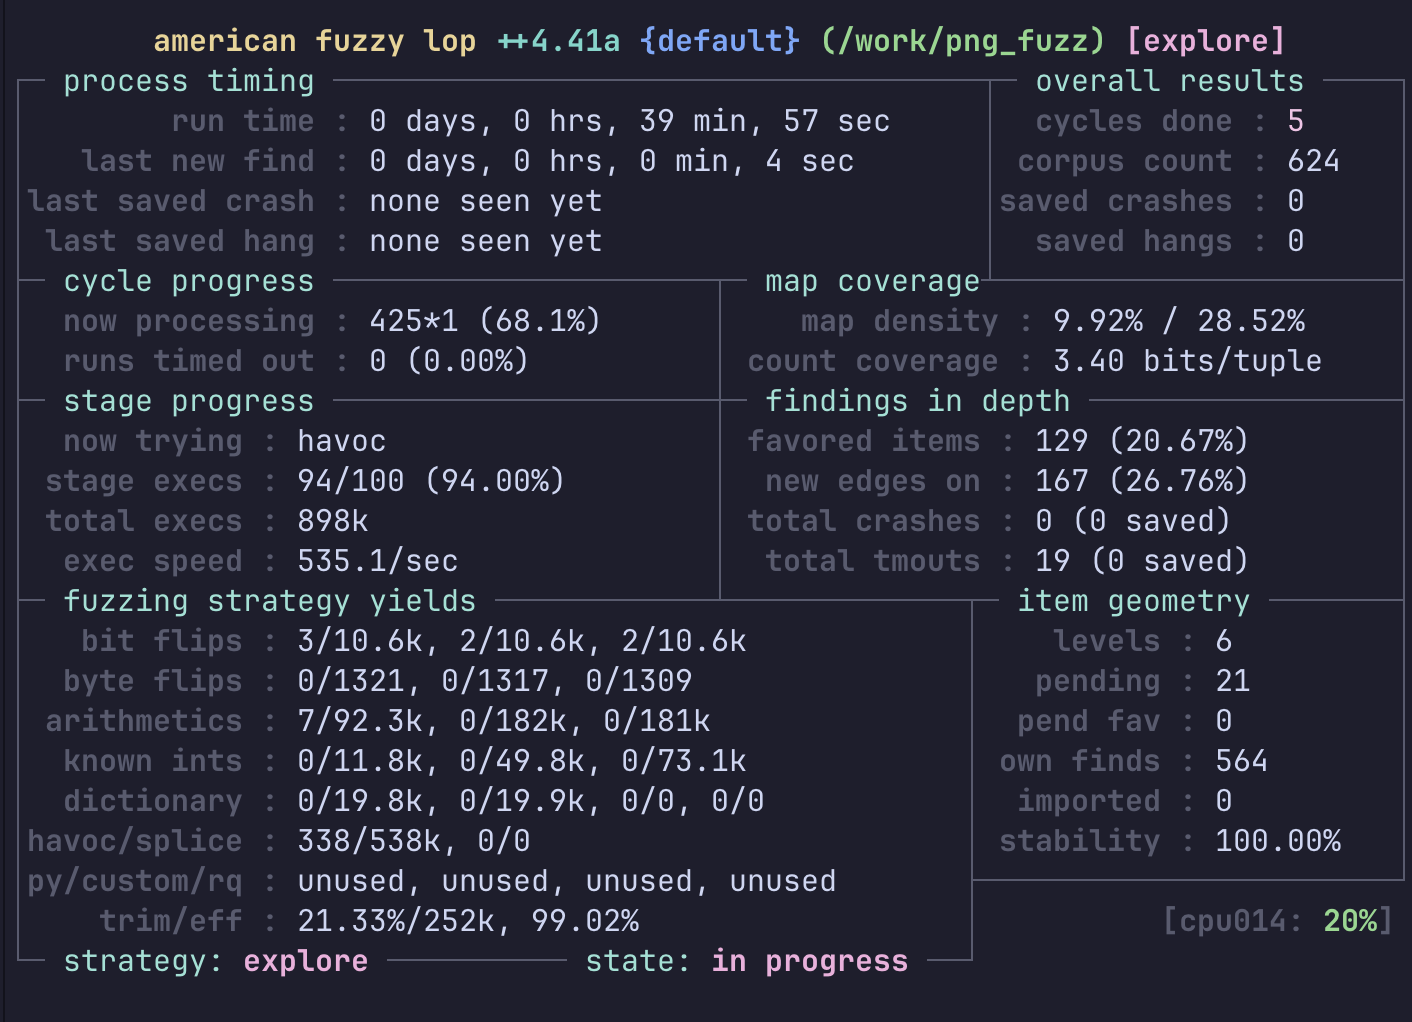
\includegraphics[width=\linewidth]{figures/status_whitebox.png}
    \caption{AFL++ status screen at the end of the white-box campaign (40 minutes, libpng~1.2.56).}
    \label{fig:status-whitebox}
\end{figure}

\begin{figure}[H]
    \centering
    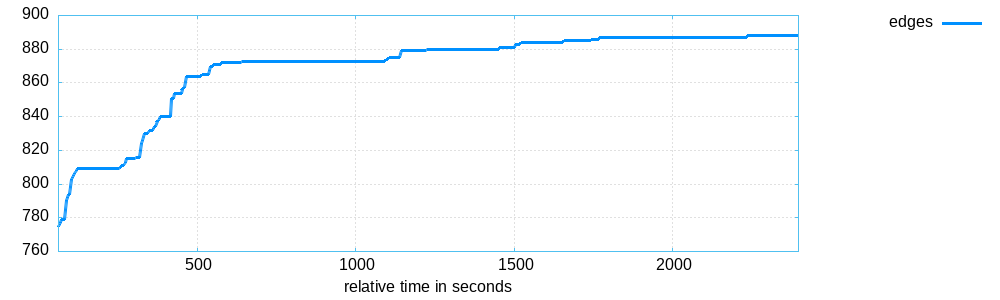
\includegraphics[width=\linewidth]{figures/edges-whitebox-40m.png}
    \caption{Edges discovered over time during the white-box campaign, generated with \texttt{afl-plot}.}
    \label{fig:edges-whitebox}
\end{figure}

%Q5
\begin{lstlisting}[language=C, caption={Synthetic off-by-one bug injected in png\_read\_info()}, label={lst:synthetic-bug}]
if (chunk_name[0] == 'I' &&
    chunk_name[1] == 'H' &&
    chunk_name[2] == 'D' &&
    chunk_name[3] == 'S')
{
    png_bytep small = (png_bytep)png_malloc(png_ptr, 4);
    small[4] = 0x41;  /* off-by-one write */
    png_free(png_ptr, small);
}
\end{lstlisting}

\begin{lstlisting}[language=bash, caption={Command to reproduce crash with ASan}, label={lst:asan-command}]
docker run --rm -v "$(pwd)":/work cs412-libpng-fuzz bash -lc '
CRASH=$(ls /work/findings/default/crashes/id:* | head -n 1)
ASAN_OPTIONS=symbolize=1:detect_leaks=0:abort_on_error=1 \
/work/png_fuzz "$CRASH"
'
\end{lstlisting}

\begin{figure}[H]
    \centering
    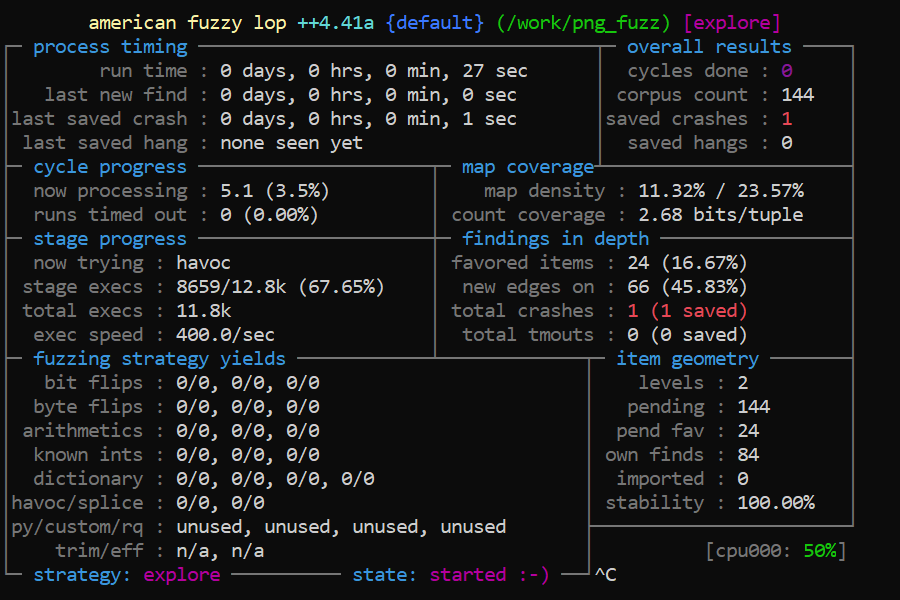
\includegraphics[width=0.95\textwidth]{figures/Afl_crash.png}
    \caption{AFL++ status screen showing the synthetic off-by-one bug detected.}
    \label{fig:afl-synthetic-crash}
\end{figure}

\begin{figure}[H]
    \centering
    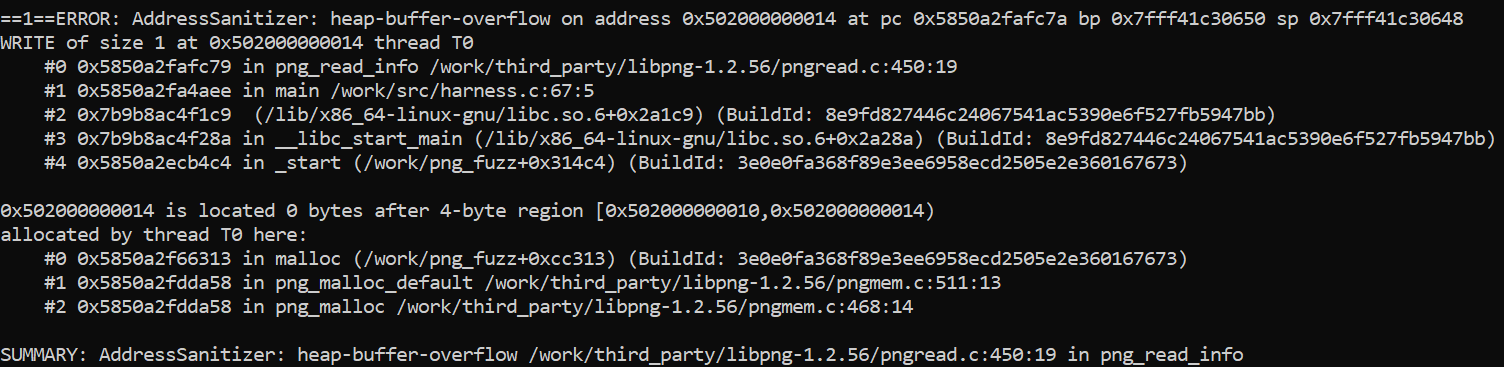
\includegraphics[width=0.95\textwidth]{figures/ASAN_crash.png}
    \caption{ASan report confirming the synthetic off-by-one bug as a heap buffer overflow inside \texttt{png\_read\_info()}.}
    \label{fig:asan-synthetic-bug}
\end{figure}

% Q7

\begin{table}[H]
\centering
\small
\begin{tabular}{l r r}
\toprule
\textbf{Metric} & \textbf{White-box} & \textbf{QEMU} \\
\midrule
Wall-clock time     & 2397 s          & 2398 s \\
Exec speed          & 535.1 exec/s    & 440.74 exec/s \\
Total executions    & 898k            & 1.06M \\
Edges discovered    & 888 / 3114      & 2375 / 65536 \\
Corpus count        & 624             & 703 \\
Map density         & 28.52\%         & 3.62\% \\
Cycles done         & 5               & 6 \\
Stability           & 100.00\%        & 100.00\% \\
Target mode         & \texttt{default} & \texttt{qemu} \\
\bottomrule
\end{tabular}
\caption{Comparison between the white-box and binary-only QEMU-mode campaigns. Values are taken from the AFL++ screenshots when visible; the QEMU average speed is taken from the internal logs because the status screen was temporarily idle and displayed \texttt{0.00 exec/s}.}
\label{tab:q7-qemu-comparison}
\end{table}


\begin{figure}[H]
    \centering
    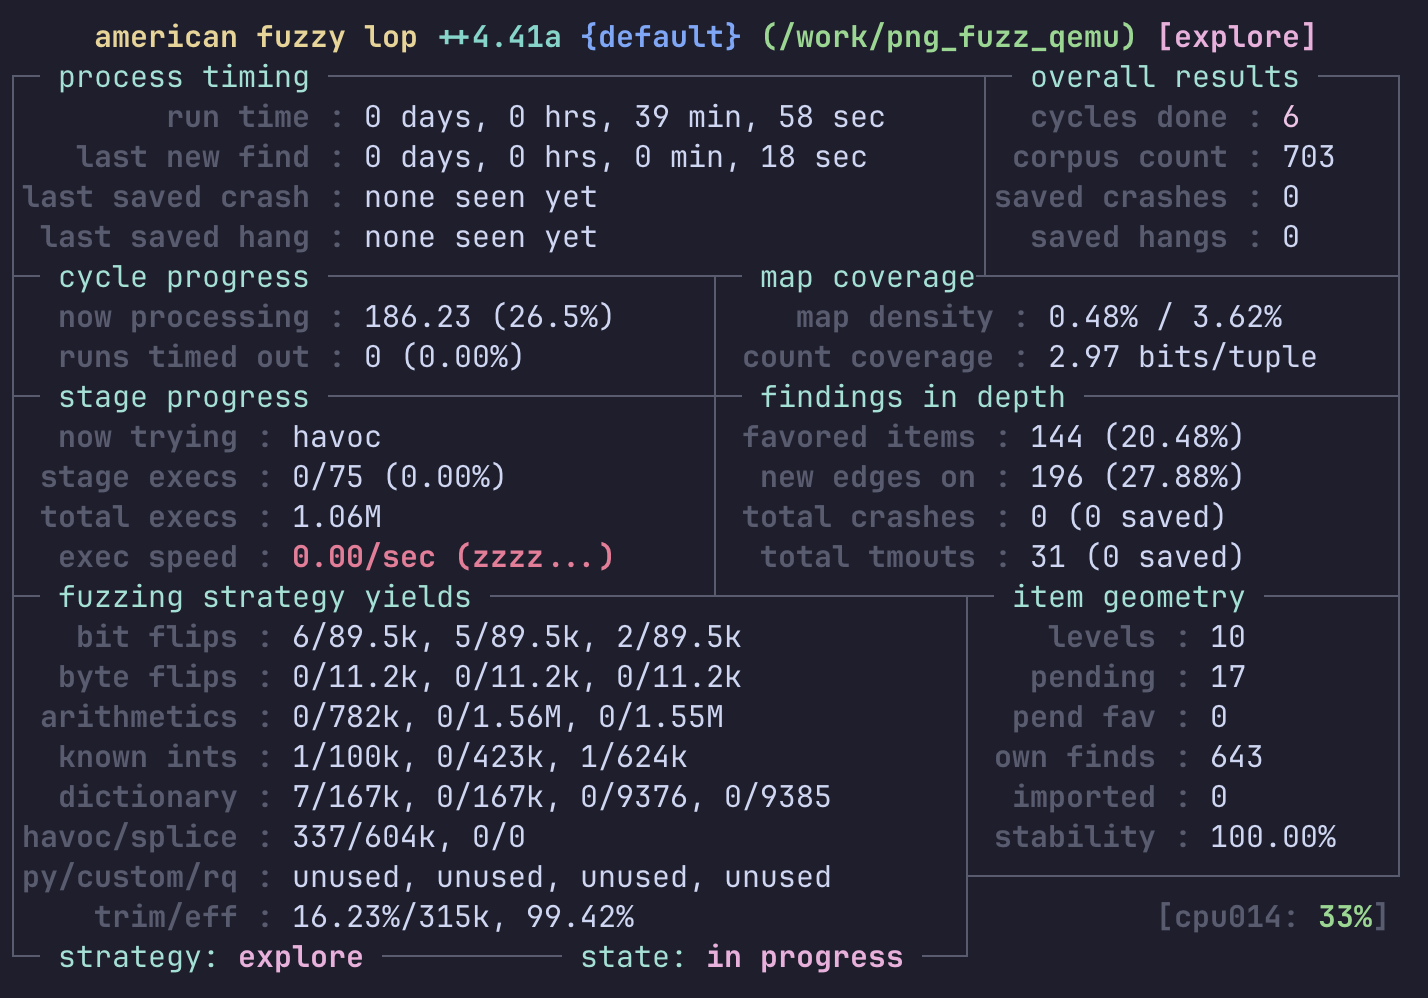
\includegraphics[width=\linewidth]{figures/status_qemu.png}
    \caption{AFL++ status screen at the end of the binary-only QEMU-mode campaign (40 minutes, libpng~1.2.56).}
    \label{fig:status-qemu}
\end{figure}


\begin{figure}[H]
    \centering
    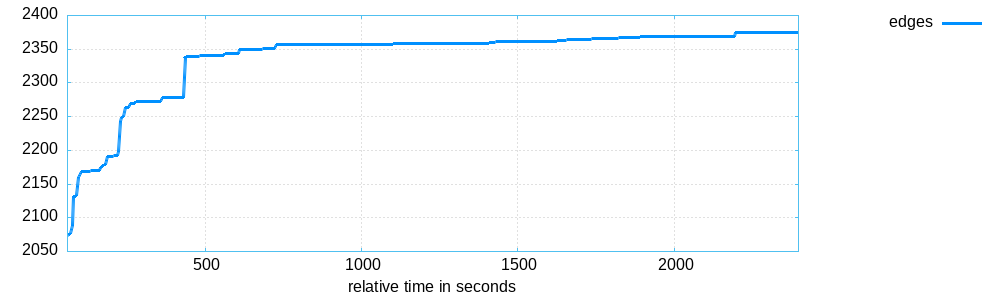
\includegraphics[width=\linewidth]{figures/edges-qemu-40m.png}
    \caption{Edges discovered over time during the binary-only QEMU-mode campaign, generated with \texttt{afl-plot}.}
    \label{fig:edges-qemu}
\end{figure}



% Q8

\begin{table}[H]
\centering
\small
\begin{tabular}{l r r r}
\toprule
\textbf{Target} &
\textbf{Total edges} &
\textbf{Reached} &
\textbf{Peak density} \\
\midrule
libpng via \texttt{pngtest\_libpng\_asan} & 4288 & $\approx$1149 & 26.8\% \\
final harness \texttt{png\_fuzz} & 3114 & $\approx$660 & 21.2\% \\
\bottomrule
\end{tabular}
\caption{Instrumentation-depth comparison between libpng's own driver and the final fuzzing harness. Peak densities are taken from the AFL++ screenshots; total edge counts are taken from internal logs.}
\label{tab:q8-instrumentation-depth}
\end{table}


\begin{table}[H]
\centering
\small
\begin{tabular}{l r r l}
\toprule
\textbf{Configuration} &
\textbf{Speed} &
\textbf{Execs} &
\textbf{Notes} \\
\midrule
No sanitizer + fork mode &
1212.97 exec/s &
363913 &
Fast fork-mode baseline; values from internal logs due to UI/capture issue \\

ASan + fork mode &
529.1 exec/s &
32.0k &
Slower due to sanitizer overhead; value visible in the screenshot \\

ASan + persistent mode &
1372 exec/s &
82.2k &
Fastest because persistent mode avoids most fork/exec reset cost \\
\bottomrule
\end{tabular}
\caption{Performance comparison of the final harness under different fuzzing 
configurations. Screenshot values are used when available; the no-sanitizer fork-mode values are taken from internal logs because the corresponding UI screenshot was incorrect.}
\label{tab:q8-performance}
\end{table}

\begin{figure}[H]
    \centering
    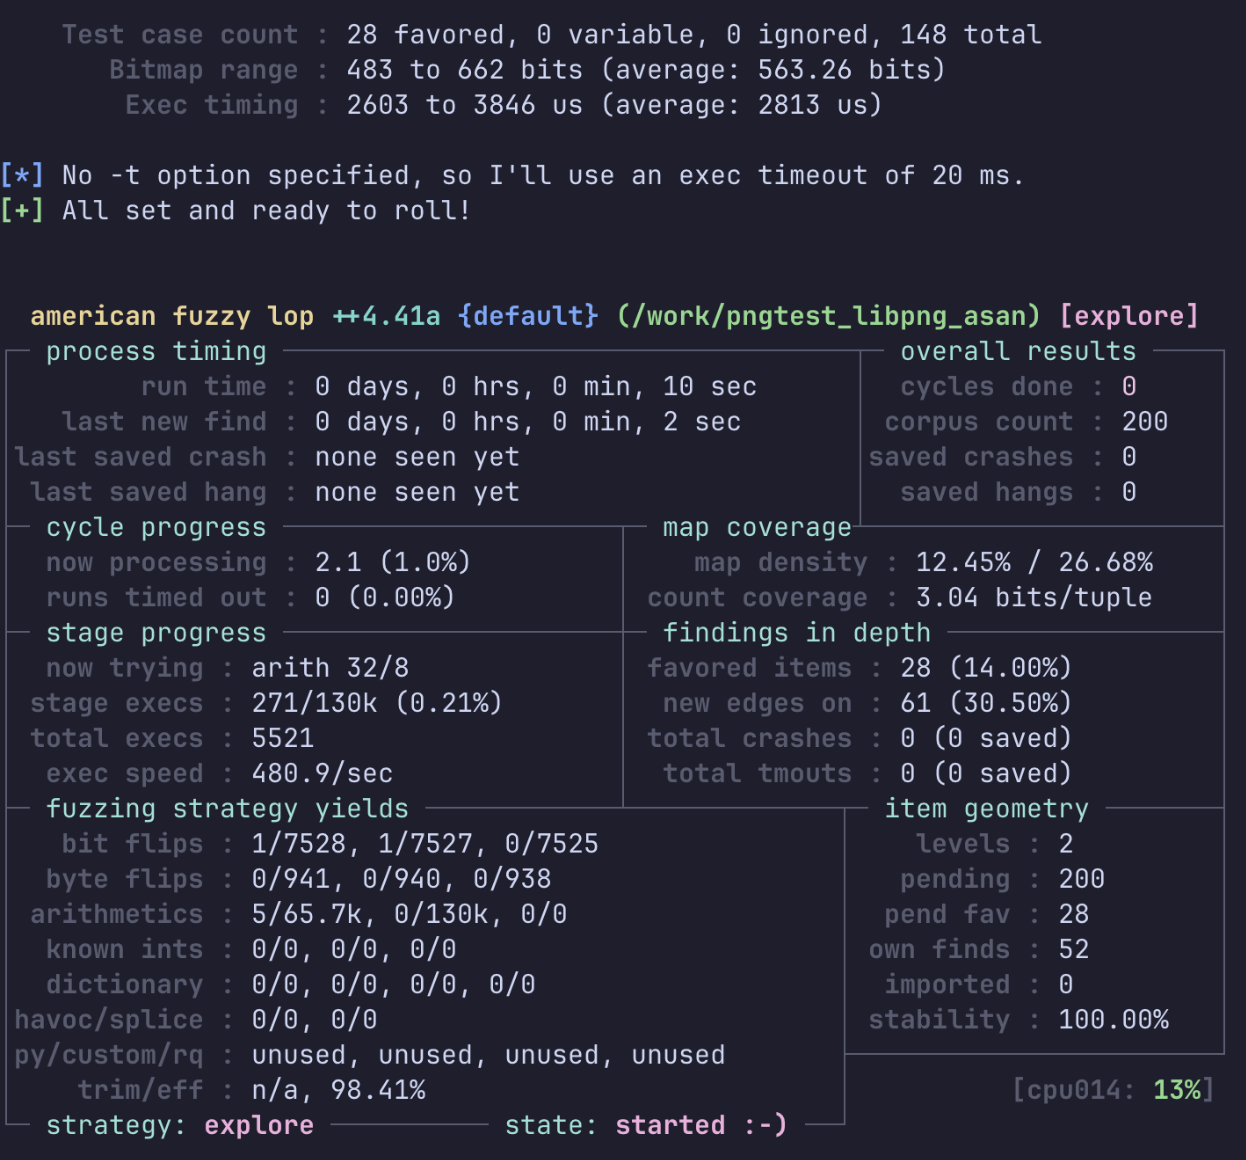
\includegraphics[width=0.95\textwidth]{figures/q8_edges_libpng.png}
    \caption{AFL++ startup screen for \texttt{pngtest\_libpng\_asan}, reporting the total instrumented edge count for the libpng driver.}
    \label{fig:q8-edges-libpng}
\end{figure}

\begin{figure}[H]
    \centering
    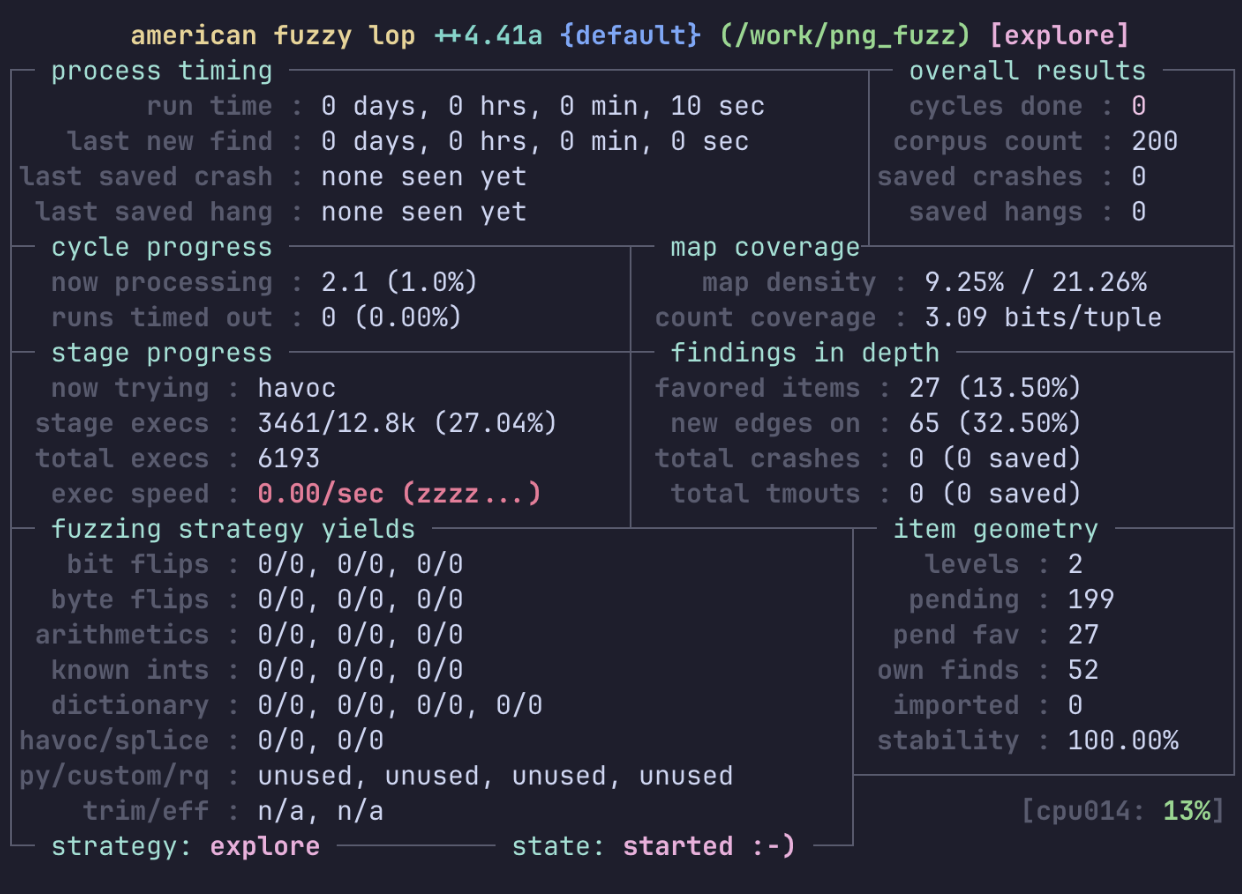
\includegraphics[width=0.95\textwidth]{figures/q8_edges_harness.png}
    \caption{AFL++ startup/status screen for the final \texttt{png\_fuzz} harness, reporting the total instrumented edge count for the fuzzing harness.}
    \label{fig:q8-edges-harness}
\end{figure}

\begin{figure}[H]
    \centering
    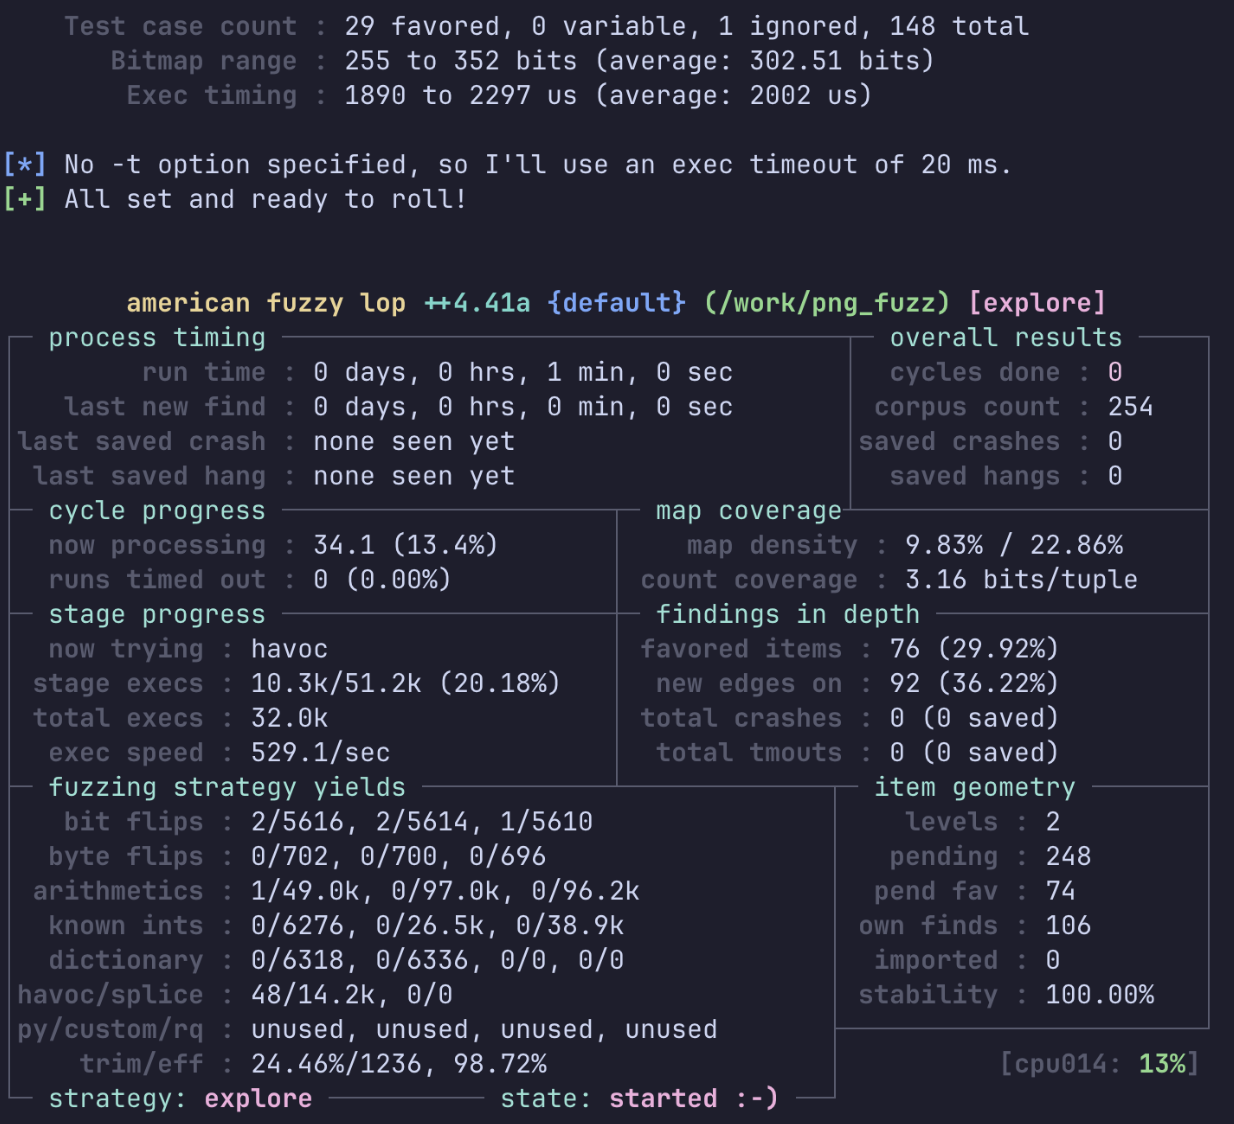
\includegraphics[width=0.95\textwidth]{figures/q8_speed_asan_fork.png}
    \caption{AFL++ status screen for the ASan fork-mode performance measurement.}
    \label{fig:q8-speed-asan-fork}
\end{figure}

\begin{figure}[H]
    \centering
    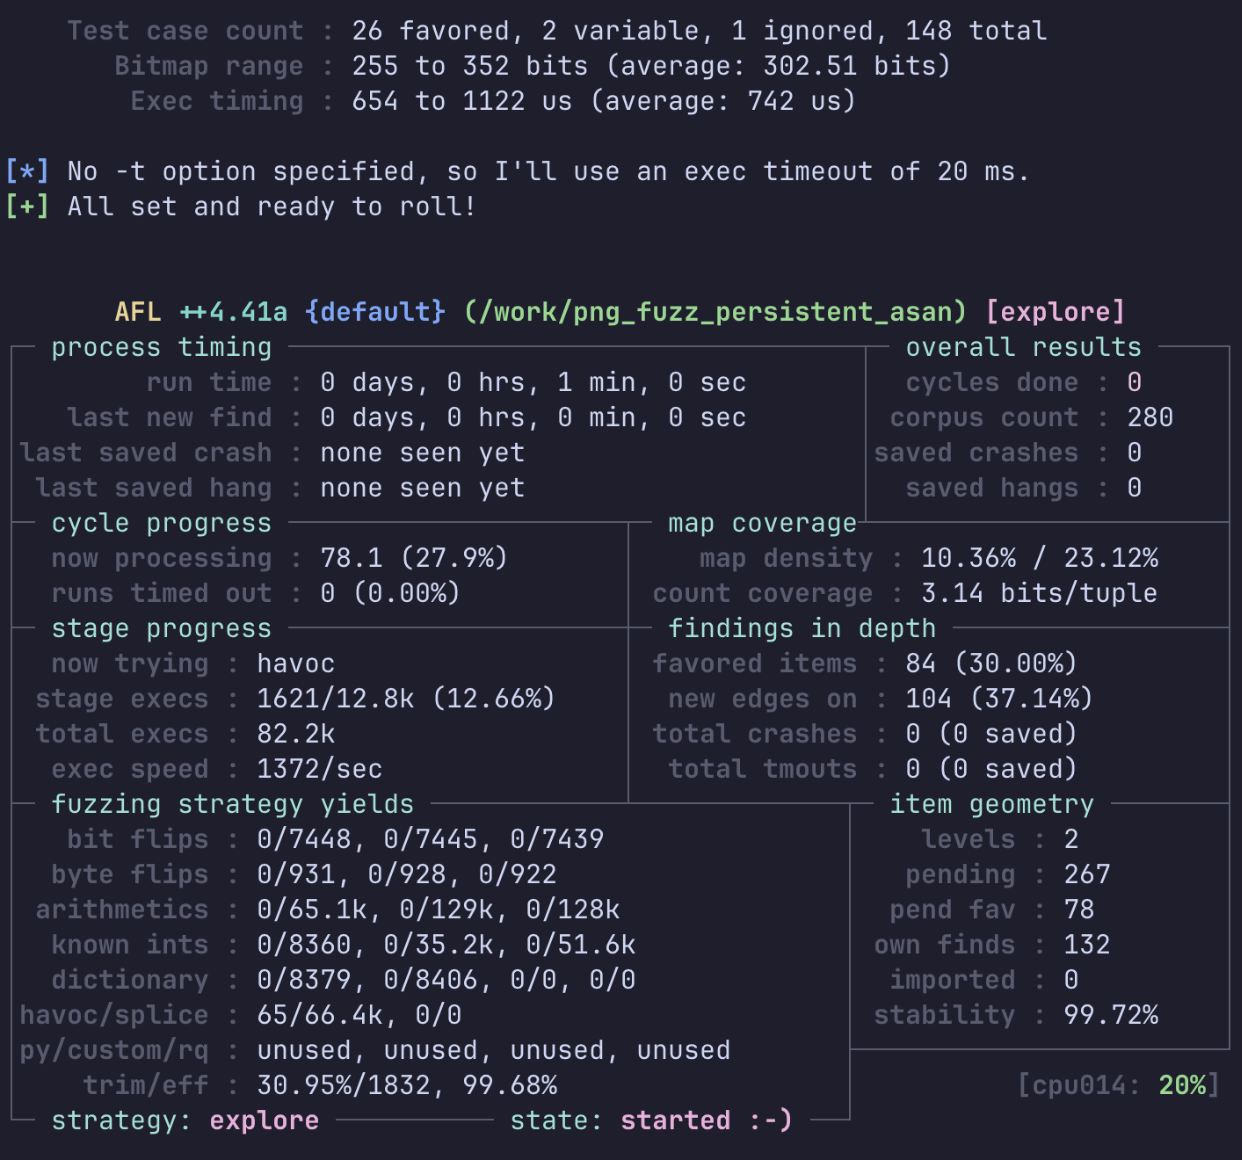
\includegraphics[width=0.95\textwidth]{figures/q8_speed_asan_persistent.png}
    \caption{AFL++ status screen for the ASan persistent-mode performance measurement.}
    \label{fig:q8-speed-asan-persistent}
\end{figure}


\newpage

{\footnotesize \bibliographystyle{acm}
\bibliography{bibliography}}

\end{document}







